\section{Fondamentaux}
Cette section parcourt les notions fondamentales d'optique pour comprendre la suite de ce rapport.

\subsection{Le seeing astronomique}
Le seeing, de l'anglais du mot vision (plutôt de l'action de voir), est le mot utilisé pour parler de la dégradation de l'image
d'un objet astronomique par les turbulences atmosphériques, plus concrètement cela se traduit pour un effet de flou et de distorsion sur l'image.

L'atmosphère est composée de plusieurs couches d'air aux densités et températures différentes, qui ont pour effet de modifier leurs coefficients de réfraction, la lumière devra donc passer
dans des couches aux indices de réfraction différents, causant alors des réfractions de la lumière non uniformes.

Le seeing peut être quantifié en seconde d'arc du disque de seeing, le diamètre de ce disque est égal à la \textbf{largeur à mis-hauteur} de l'intensité lumineuse :
\begin{figure}[H]
  \centering
  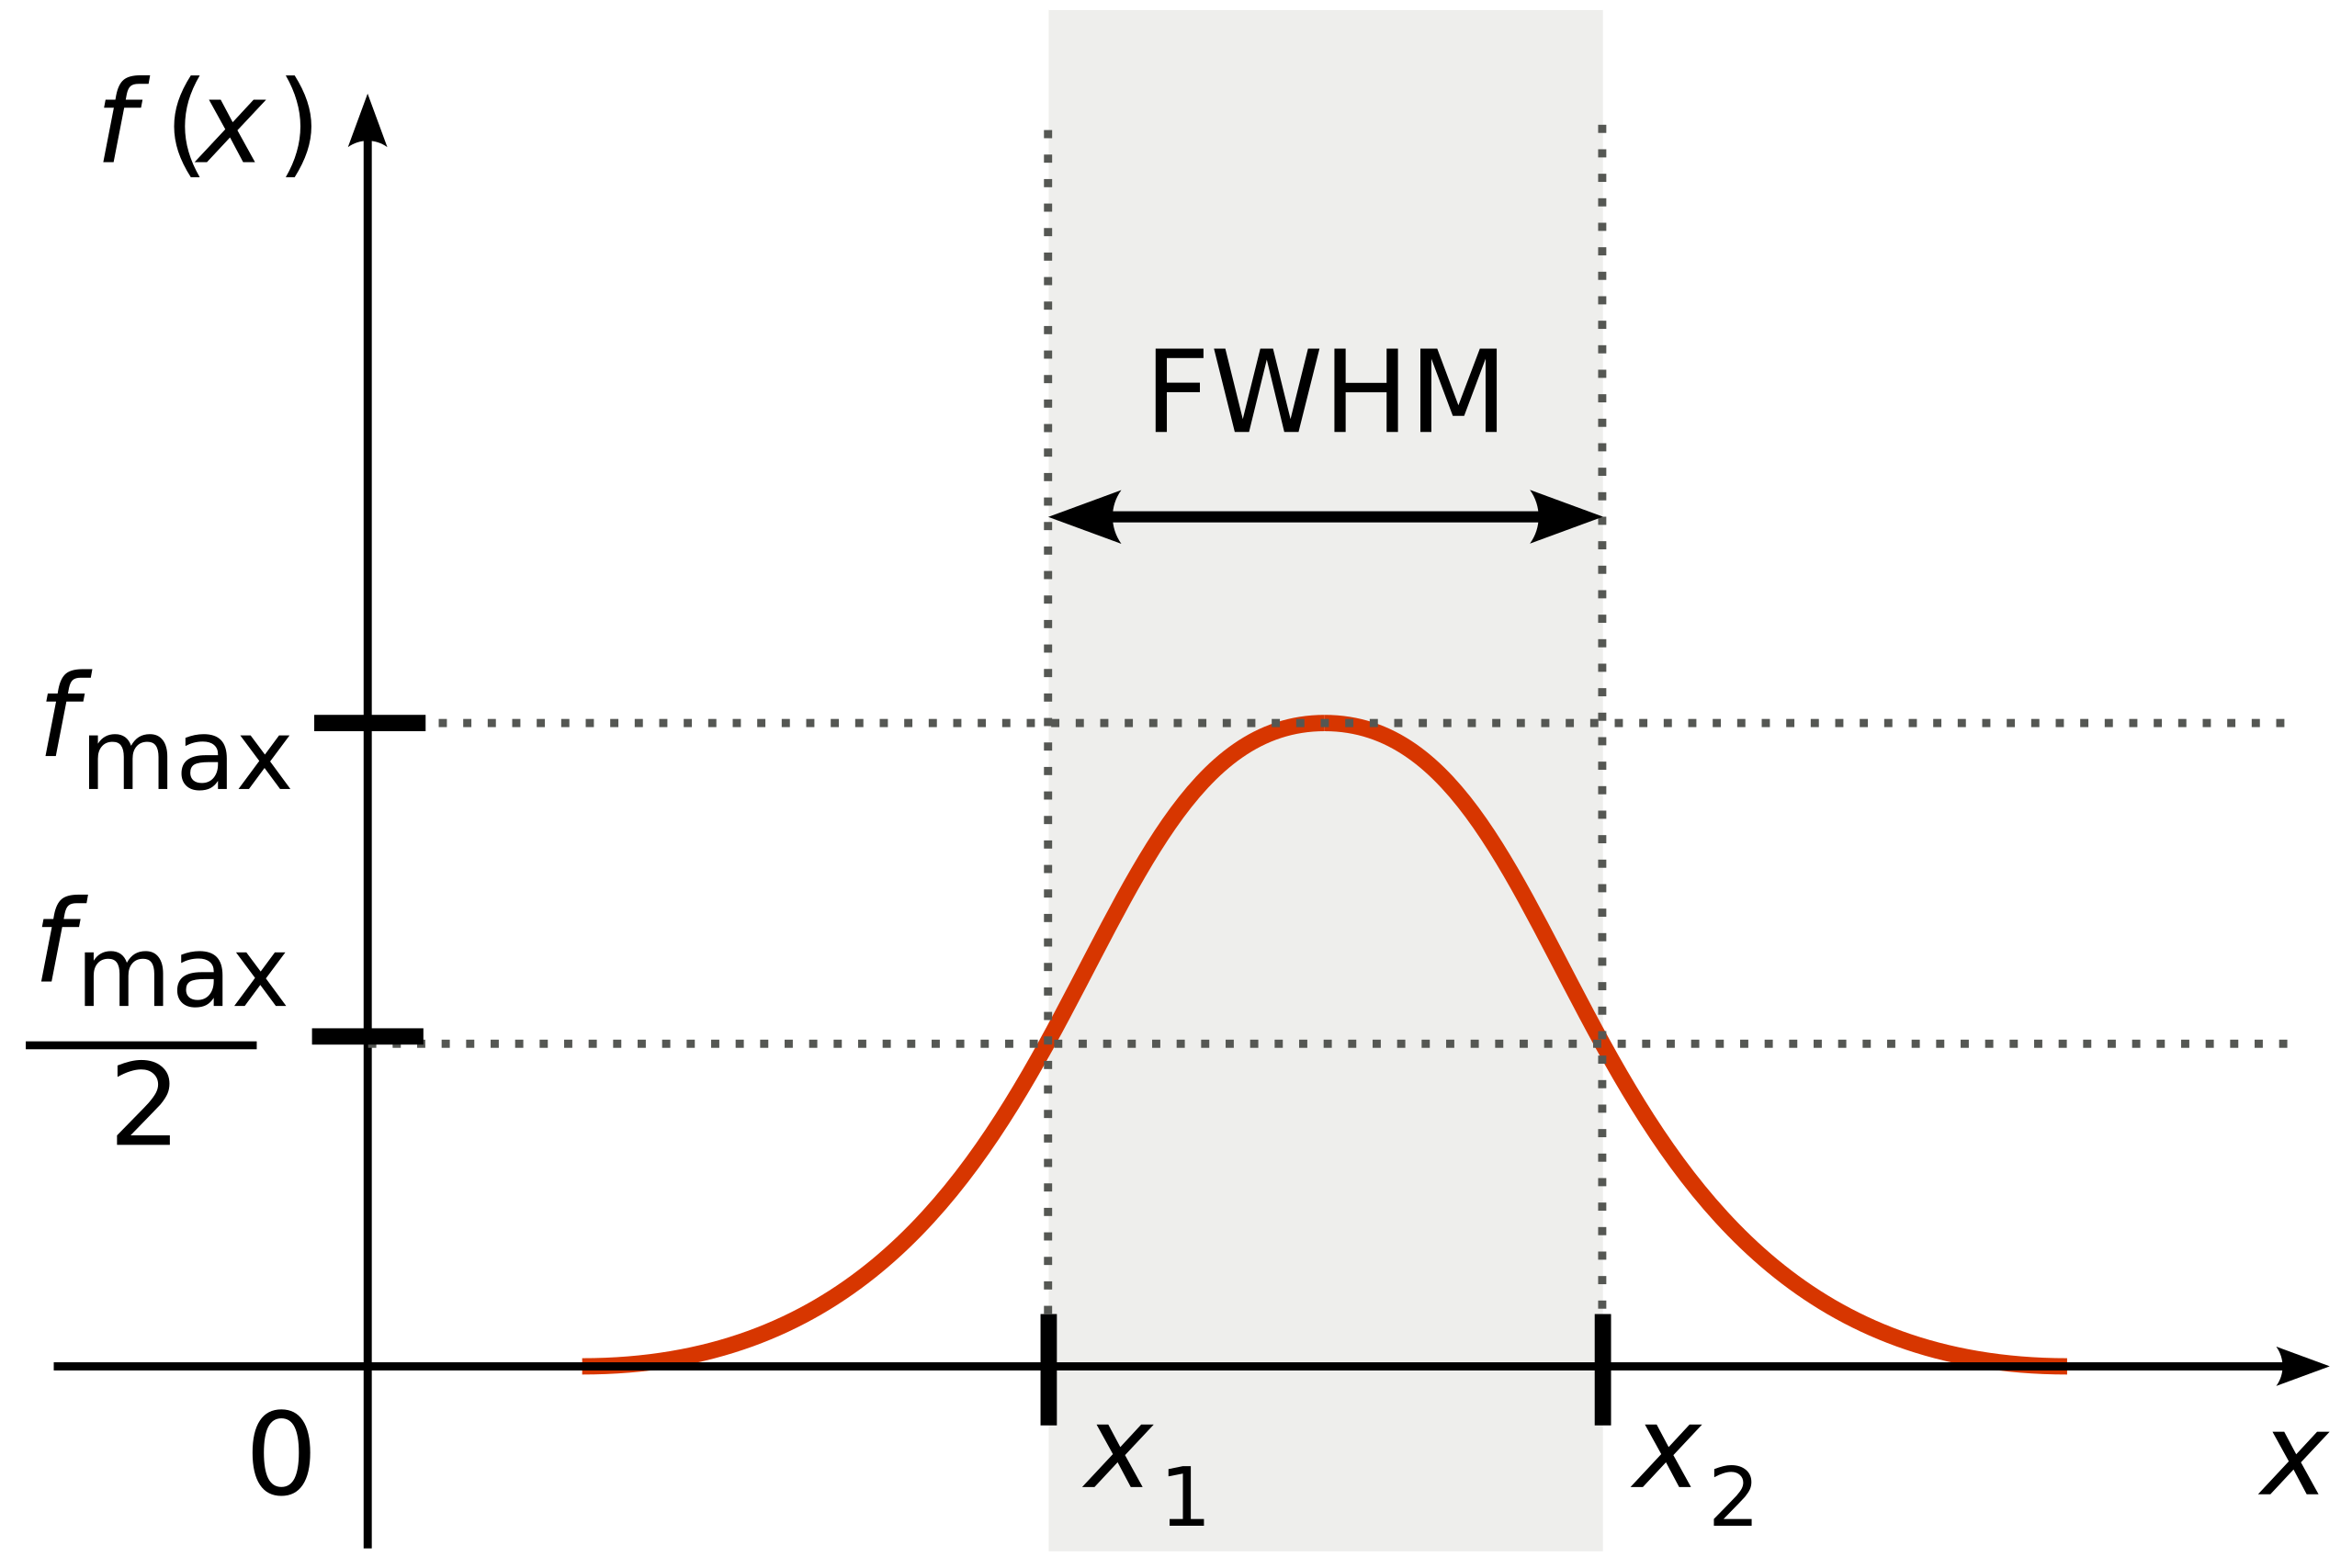
\includegraphics[width=0.5\textwidth]{assets/figures/théorie/FWHM.png}
  \caption[Illustration de la LMH]{Illustration de la largeur à mi-hauteur \autocite{largeur_mis_hauteur}\footnotemark}\label{fig:largeur_mis_hauteur}
\end{figure}

\footnotetext{\fullcite{largeur_mis_hauteur}}
Un seeing étant $\leq  0.4$" d'arc est considéré comme excellent, au DAG le seeing est usuellement de 0.9".

Une autre façon de quantifier le seeing est le paramètre de Fried $\mathbf{r_0}$. Pour expliquer le paramètre $r_0$, c'est le diamètre en cm qu'aurait un télescope
qui fournirait, en l'absence de turbulences, la même image que notre télescope en présence de turbulences. C'est ce paramètre $r_0$ qui sera utilisé en suite pour caractériser les écrans de phase.

La formule qui sera utilisée dans le calcul du paramètre de Fried sera :
\begin{equation}
  \sigma_{a_j}^2 \sim F(j) \cdot (\frac{D}{r_0})^{5/3} \label{eq:param_fried}
\end{equation}

Où :
\begin{itemize}
  \item $\sigma_{a_j}^2$ = la variance des coefficients de Zernike j
  \item  $F(j)$ = variance des coefficients de Zernike pour D/r0 = 1
  \item $D$ = diamètre du téléscope
  \item $r_0$ = paramètre de Fried
\end{itemize}

\subsection{Les turbulences atmosphériques}

\subsubsection{Cause physique}
L'atmosphère de notre planète n'est pas un bloc homogène, cette dernière est composée de \textbf{masses d'air}. Ces masses d'air
sont des zones de l'atmosphère où les conditions de température, de pression et d'humidité sont homogènes \cite{masse_air_wiki}\cite{masse_air_unige}.
L'écoulement de ces zones se fait en régime turbulent à des vitesses usuellement mesurées entre 1 et 20 m/s sur des longueurs de 10 à 1000m, ce phénomène
turbulent des mouvements de masses d'air sera qualifié de \textbf{turbulence dynamique} dans la suite de ce rapport.

Cette turbulence dynamique (la vitesse de l'écoulement) n'a pas d'incidence directe sur la propagation des ondes lumineuses, seul l'indice de réfraction de l'atmosphère influence la propagation
de la lumière. L'indice de réfraction est influencé par la densité de l'air selon la loi de Dale-Gladstone:

% \begin{equation}
%     N = 77.6 (\frac{P}{T}) + 3.74\cdot 10^5 (\frac{e}{T^2}) + C\frac{n_e}{f^2}
% \end{equation}

% Où:
% \begin{itemize}
%     \item $P$ = pression exprimée en hPa
%     \item $T$ = température absolue (K)
%     \item $e$ = pression de vapeur d'eau contenue dans l'air (hPa)
%     \item $C$ = $4,03 \cdot 10^{-7} m^{-3}Hz^2$
%     \item $n_e$ = densité électronique
%     \item $f$ = fréquence du signal
% \end{itemize}

\begin{equation}
  n-1 \sim \rho = \alpha_n \cdot \frac{P}{T}
\end{equation}

Où:
\begin{itemize}
  \item $P$ = pression exprimée en $N/m^2$
  \item $T$ = température absolue (K)
  \item $\alpha_a$ = $80\cdot10^{-8} K/Pa$
\end{itemize}

Pour aller plus loin, c'est généralement la température qui aura une grande influence sur l'indice de réfraction de l'air
et non la pression, car cette dernière est constante dans toute l'épaisseur d'une couche turbulente. Cette perturbation d'indice de
réfraction entre les couches turbulentes est donc la source des \textbf{Turbulences optiques}\cite{thèse_laurent_turbulence}.

\newpage
\subsubsection{Types de turbulences}
Plusieurs types de turbulences optiques sont observables à des altitudes bien spécifiques,
il est possible d'en distinguer 4 types :

\say{

  \begin{itemize}
    \item \textbf{1. Turbulence de coupole :}
          \newline
          Elle apparaît lorsque l'air n'a pas la même température à l'intérieur et à l'extérieur de la coupole (du télescope). Cette dernière
          correspond à la turbulence du miroir.

    \item \textbf{2. Turbulence de surface :}
          \newline
          Active sur les premiers 10 à 100m. Elle doit son origine au refroidissement par convection du sol chauffé par le rayonnement solaire.
          Typiquement, elle atteint un minimum juste après le lever du soleil, puis augmente régulièrement jusqu'au début de l'après-midi. Elle décroit
          ensuite pour atteindre un second minimum après le coucher du soleil, puis augmente légèrement durant la nuit. Le moyen de minimiser au maximum cette turbulence
          est le choix du site d'installation du télescope. Par exemple, placer le télescope en haut d'une tour loin de toute surface minimisera le phénomène.

    \item \textbf{3. Turbulence de moyenne altitude 1-5/6 Km :}
          \newline
          Elle trouve son origine à la fois dans les perturbations orographiques (ondes générées par les reliefs) des courants atmosphériques et dans les instabilités thermiques
          de l'atmosphère. Elle est constituée par une multitude de fines couches turbulentes de quelques centaines de mètres d'épaisseur. Ici encore, seule la sélection du site d'accueil est susceptible
          de minimiser cette composante.

    \item \textbf{4. Turbulence de tropopause et stratosphérique :}
          \newline
          Au-delà de $\approx 6 $Km, on observe une certaine systématique pour la plupart des sites :
          la turbulence atteint un minimum entre 6 et 10 Km, puis augmente à nouveau pour atteindre un maximum dans la tropopause (zone de transition entre la troposphère et la stratosphère), 10-20 Km. Cette couche
          turbulente est due à la présence de forts vents cisaillant l'atmosphère, très fréquents à la limite de la troposphère. La turbulence optique diminue en suite dans la stratosphère, pour finalement disparaître
          au-delà de 25 à 30 Km d'altitude.
  \end{itemize}

} \footnotemark


\footnotetext{\cite{thèse_laurent_turbulence_types}\fullcite{thèse_laurent_turbulence_types}}

\newpage
\subsubsection{Illustration des effets des turbulences}

Pour illustrer concrètement les effets des turbulences, ainsi que donner une idée de l'impact de la valeur du seeing sur la PSF\footnotemark (Point Spead Function) d'un télescope
:
\begin{figure}[H]
  \centering
  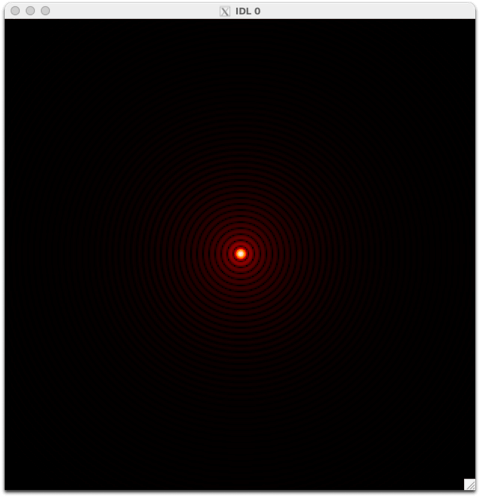
\includegraphics[width=0.5\textwidth]{assets/figures/théorie/PSF_parfaite.png}
  \caption[PSF parfaite]{PSF parfaite d\textquotesingle un télescope de 1m de diamètre, longueur d'onde 500 nm}
\end{figure}

\begin{figure}[H]
  \centering
  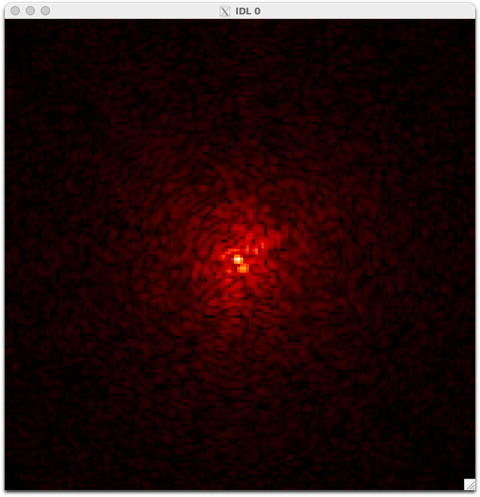
\includegraphics[width=0.5\textwidth]{assets/figures/théorie/PSF_seeing_1second.png}
  \caption[PSF avec seeing 1"]{PSF du même télescope, avec image instantanée pour un seeing de 1"}
\end{figure}
\footnotetext{La PSF décrit la distribution d\textquotesingle intensité de la lumière provenant d\textquotesingle un point source.}
\begin{figure}[H]
  \centering
  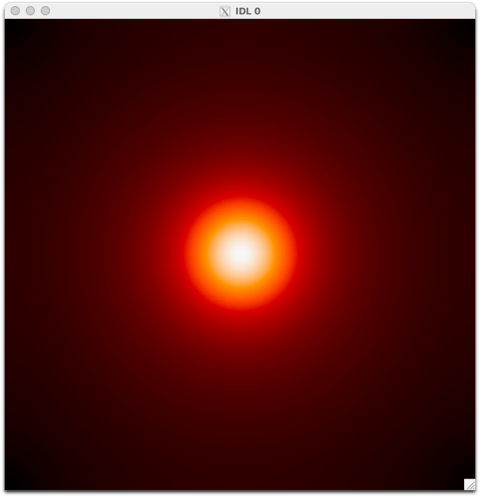
\includegraphics[width=0.5\textwidth]{assets/figures/théorie/PSF_turbulente.png}
  \caption[PSF turbulente]{PSF turbulente, longue exposition}
\end{figure}

Il est donc possible d'observer l'impact de la turbulence sur une image instantanée et sur une image à longue exposition, cela résultera en une perte de détails et donc à une image
finale beaucoup plus douce.


\subsection{Front d'onde et coefficients de Zernike}
\subsubsection{Front d'onde}
Un front d'onde est une surface imaginaire qui relie tous les points d'une onde ayant la même phase à un instant donné.
Pour la lumière, cela signifie que tous les points sur un front d'onde ont parcouru la même distance depuis la source lumineuse et oscillent en phase.
Le front d'onde est perpendiculaire à la direction de la lumière, donc une réfraction modifiera de manière prédictible le front d'onde :

\begin{figure}[H]
  \centering
  \begin{subfigure}{.5\textwidth}
    \centering
    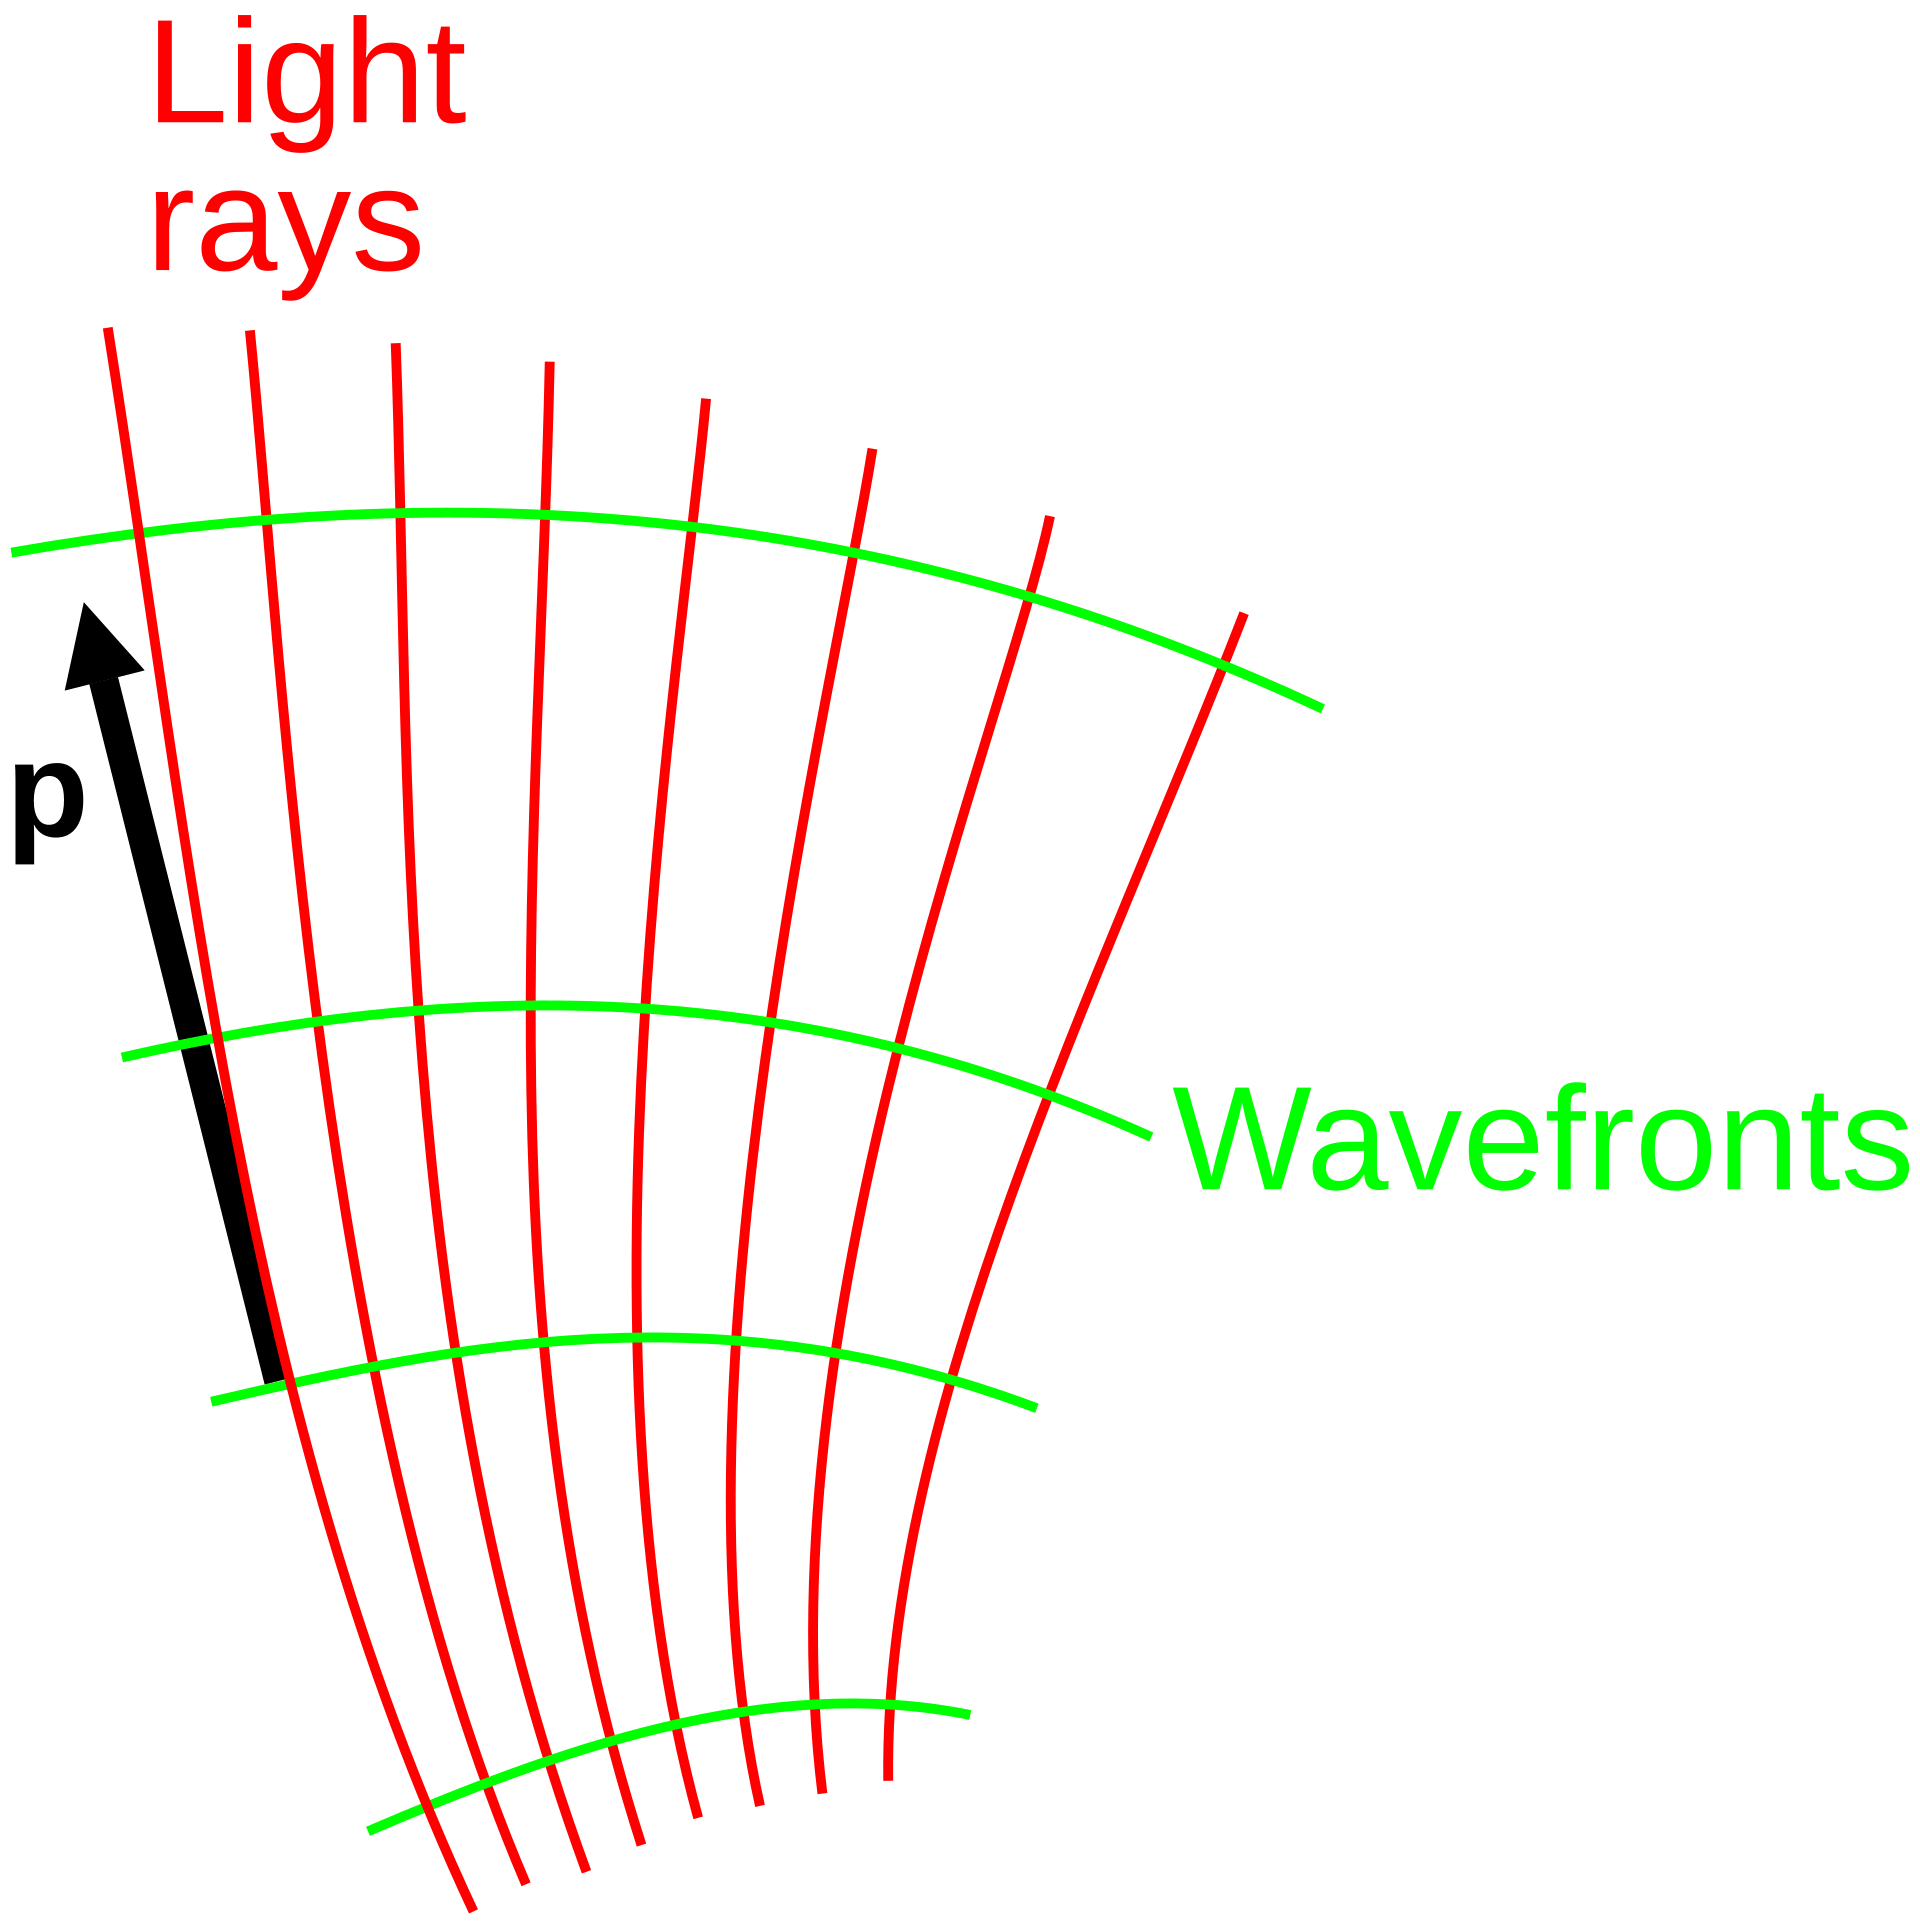
\includegraphics[width=.75\linewidth]{assets/figures/théorie/wavefront_representation.png}
    \caption{Représentation du front d'onde perpendiculaire}
    \label{fig:front_onde_perp}
  \end{subfigure}%
  \begin{subfigure}{.5\textwidth}
    \centering
    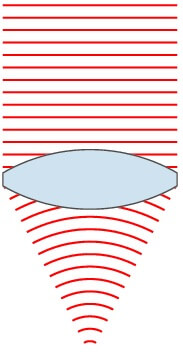
\includegraphics[width=.4\linewidth]{assets/figures/théorie/Lens_and_wavefronts.jpeg}
    \caption{Modification du front d'onde après réfraction}
    \label{fig:refraction_front_onde}
  \end{subfigure}
  \caption[Illustration front d'onde]{Illustrations du principe de front d'onde \cite{wavefront_wikipedia}\footnotemark}
  \label{fig:illu_front_onde}
\end{figure}
\footnotetext{\fullcite{wavefront_wikipedia}}

\subsubsection{Mesure du front d'onde}

Pour mesurer le front d'onde, on emploie un \textbf{capteur de front d'onde Shack-Hartmann} du fabricant Thorlabs:

\begin{figure}[H]
  \centering
  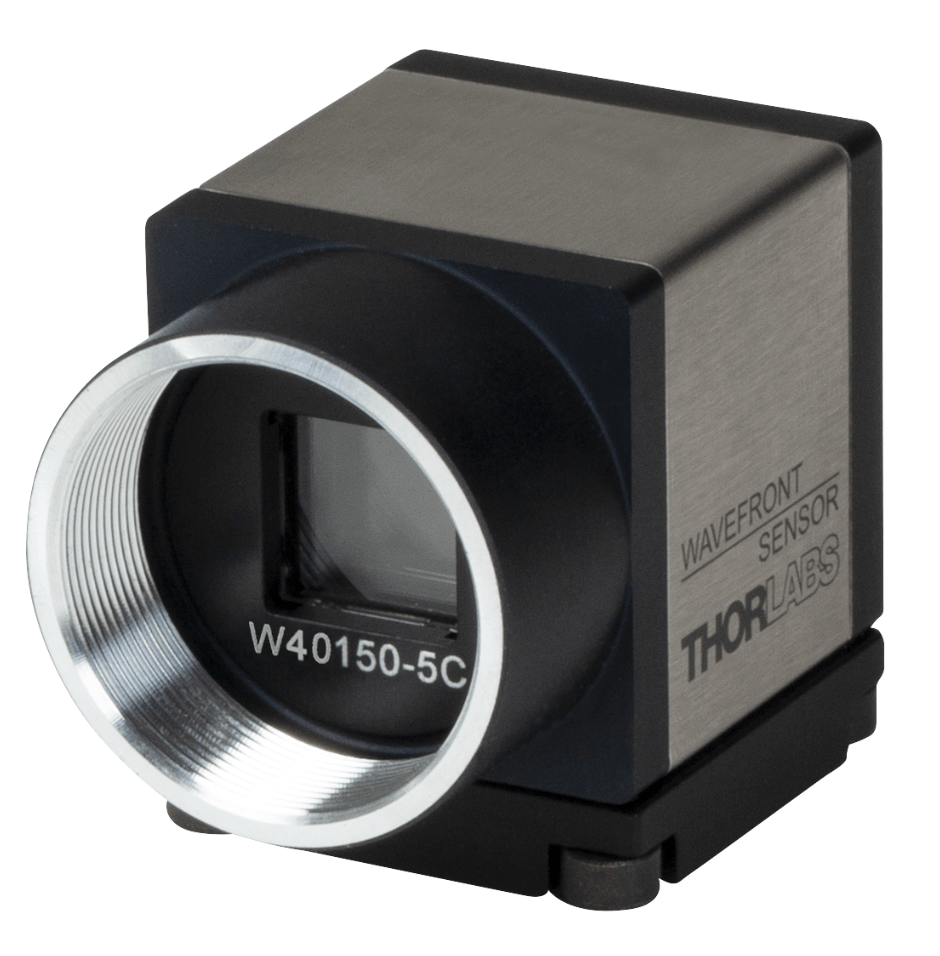
\includegraphics[width = 0.4\textwidth]{assets/figures/théorie/WFS40_7AR.png}
  \caption[Fonctionnement WFS Thorlabs]{Fonctionnement du capteur de front d'onde\cite{WFS_thorlabs_site}\footnotemark}
  \label{fig:WFS_thorlabs_fonctionnement}
\end{figure}
\footnotetext{\fullcite{WFS_thorlabs_site}}


Le principe de fonctionnement d'un capteur de Shack-Hartmann est le suivant :

\begin{figure}[H]
  \centering
  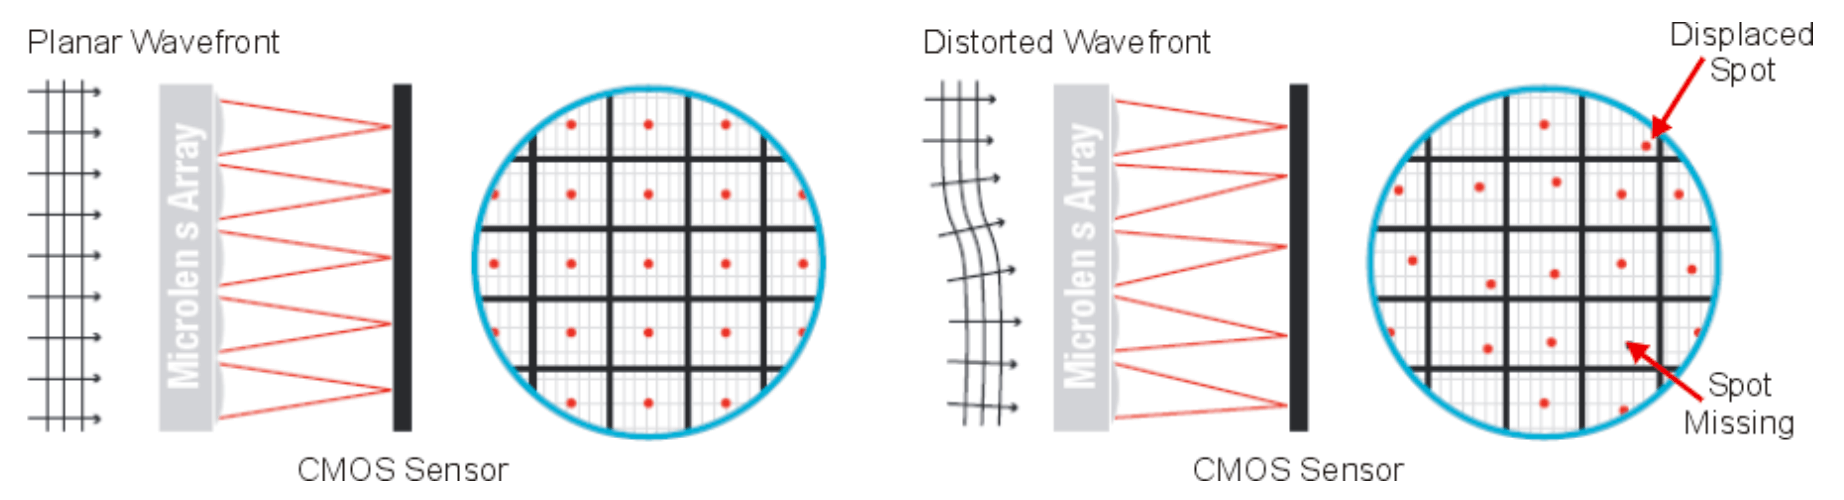
\includegraphics[width = 1.1\textwidth]{assets/figures/théorie/Shack_Hartmann_Wavefront_Distorted.png}
  \caption[Image WFS Thorlabs]{WFS4\_7AR de Thorlabs\cite{WFS_thorlabs_site}\footnotemark}
  \label{fig:WFS_thorlabs}
\end{figure}
\footnotetext{\fullcite{WFS_thorlabs_site}}

\say{ Un capteur de Shack-Hartmann consiste en une grille de lentilles et une caméra. Quand un front d'onde entre dans la matrice de lentilles,
  un champ de points est créé sur la caméra. La position de chaque point est analysée pour mesurer dynamiquement le front d'onde
  de sources laser ou pour caractériser la distorsion de front d'onde causée par des composants optiques. }\footnotemark[5]

Ce capteur nous est donc utile, car ce dernier permet de mesurer et de représenter le front d'onde du du faisceau lumineux passant à travers la turbulence
optique, ou alors, dans notre cas, à travers l'écran de phase, il retourne aussi les coefficients de Zernike du front d'onde.

\newpage
\subsubsection{Coefficients de Zernike}

Les coefficients de Zernike sont les "poids" polynômes de Zernike, c'est-à-dire la contribution que chaque polynome a pour décrire les aberrations de front d'onde,
ces derniers
permettent de décrire n'importe quelle surface dans un domaine circulaire.
\begin{figure}[H]
  \centering
  \begin{subfigure}{.5\textwidth}
    \centering
    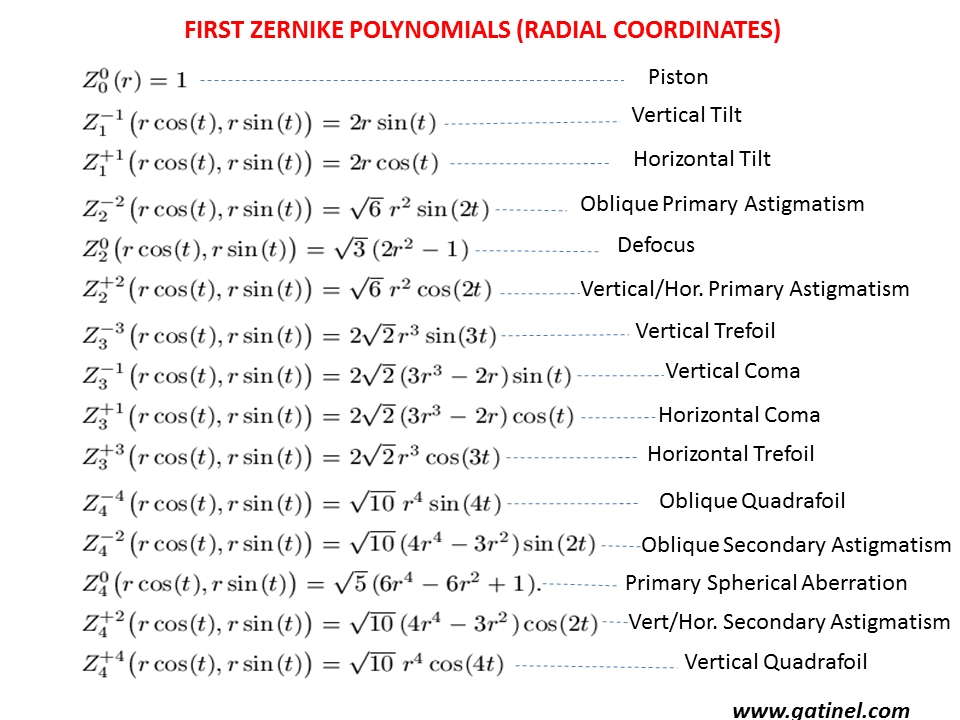
\includegraphics[width=1\linewidth]{assets/figures/théorie/Zernike-polynomials-equations.png}
    \caption{Formules des polynômes de Zernike}
    \label{fig:formules_poly_Zernike}
  \end{subfigure}%
  \begin{subfigure}{.5\textwidth}
    \centering
    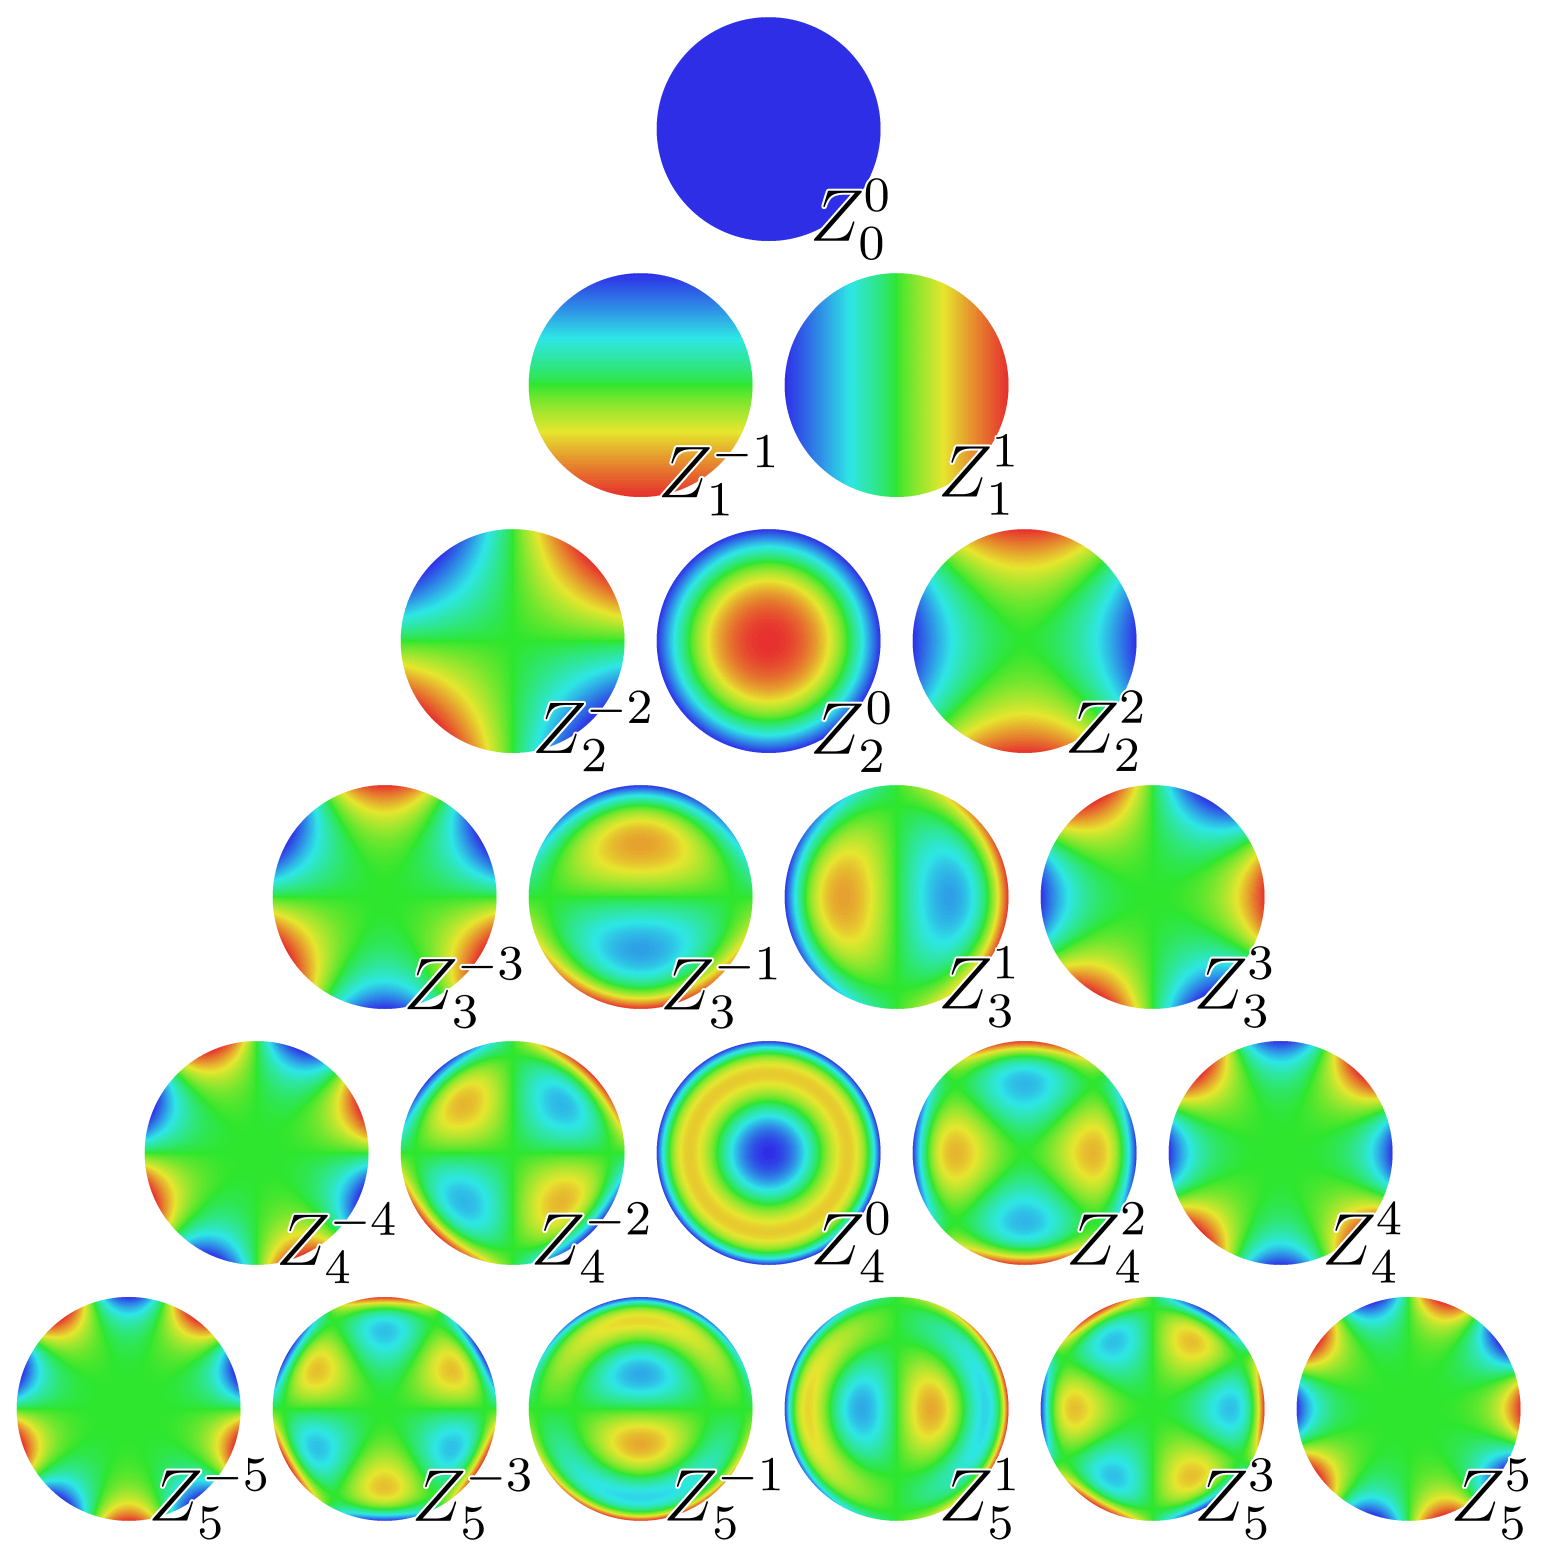
\includegraphics[width=.75\linewidth]{assets/figures/théorie/zernike_polynomes_plots.png}
    \caption{Représentation des polynômes de Zernike}
    \label{fig:plots_des_polynomes_Zernike}
  \end{subfigure}
  \caption[Illustration polynômes de Zernike]{Illustration polynômes de Zernike \cite{Zernike_docteur_Damien}\footnotemark}
  \label{fig:illu_poly_Zernike}
\end{figure}

\footnotetext{\fullcite{Zernike_docteur_Damien}}

Pour reconstruire le front d'onde il suffit alors de sommer les fronts d'ondes des coefficients de Zernike i j.